\documentclass[tikz,border=4pt]{standalone}
\usepackage[T1]{fontenc}\usepackage{helvet}\renewcommand{\familydefault}{\sfdefault}
\usepackage{xcolor}\usepackage{pgfplots}\pgfplotsset{compat=1.18}
\definecolor{rscblue}{RGB}{0,83,156}
\begin{document}
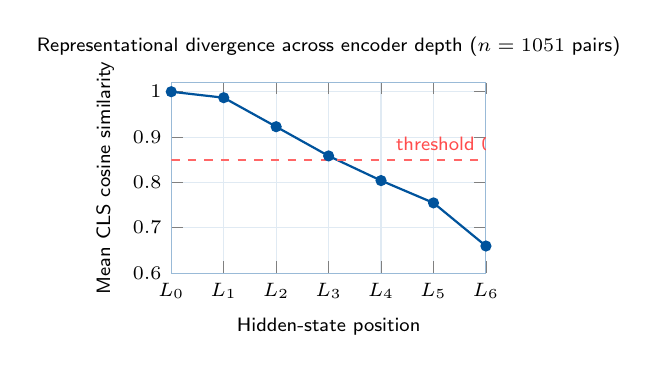
\begin{tikzpicture}
\begin{axis}[
  width=0.46\textwidth, height=4.0cm,
  xmin=0, xmax=6, ymin=0.6, ymax=1.02,
  xtick={0,1,2,3,4,5,6},
  xticklabels={$L_0$,$L_1$,$L_2$,$L_3$,$L_4$,$L_5$,$L_6$},
  ylabel={Mean CLS cosine similarity},
  xlabel={Hidden-state position},
  ylabel style={font=\scriptsize\sffamily},
  xlabel style={font=\scriptsize\sffamily},
  xticklabel style={font=\scriptsize\sffamily},
  yticklabel style={font=\scriptsize\sffamily},
  tick align=inside,
  axis line style={color=rscblue!40},
  grid=major, grid style={color=rscblue!12},
  title={\sffamily\scriptsize Representational divergence across encoder depth ($n=1051$ pairs)},
  title style={font=\scriptsize\sffamily},
]
\addplot[color=rscblue, mark=*, mark size=1.6pt, thick] coordinates {
  (0,1.0000) (1,0.9868) (2,0.9228) (3,0.8584) (4,0.8040) (5,0.7548) (6,0.6597)
};
% Divergence threshold
\addplot[color=red!60, dashed, thick, forget plot] coordinates {(0,0.85) (6,0.85)};
\node[font=\scriptsize\sffamily, color=red!70, anchor=west] at (axis cs:4.1,0.885) {threshold 0.85};
\end{axis}
\end{tikzpicture}
\end{document}
